%=======================02-713 LaTeX template, following the 15-210 template==================
%
% You don't need to use LaTeX or this template, but you must turn your homework in as
% a typeset PDF somehow.
%
% How to use:
%    1. Update your information in section "A" below
%    2. Write your answers in section "B" below. Precede answers for all
%       parts of a question with the command "\question{n}{desc}" where n is
%       the question number and "desc" is a short, one-line description of
%       the problem. There is no need to restate the problem.
%    3. If a question has multiple parts, precede the answer to part x with the
%       command "\part{x}".
%    4. If a problem asks you to design an algorithm, use the commands
%       \algorithm, \correctness, \runtime to precede your discussion of the
%       description of the algorithm, its correctness, and its running time, respectively.
%    5. You can include graphics by using the command \includegraphics{FILENAME}
%
\documentclass[11pt]{article}

\usepackage{amsmath,amssymb,amsthm}
\usepackage{graphicx}
\usepackage[margin=1in]{geometry}
\usepackage{fancyhdr}
\usepackage{comment}
\usepackage{tikz}
\usetikzlibrary{arrows}
\usepackage{caption}
\usepackage{subcaption}
\usepackage{float}


\setlength{\parindent}{0pt}
\setlength{\parskip}{5pt plus 1pt}
\setlength{\headheight}{13.6pt}
\newcommand\question[2]{\vspace{.25in}\hrule\textbf{#1: #2}\vspace{.5em}\hrule\vspace{.10in}}
\renewcommand\part[1]{\vspace{.10in}\textbf{(#1)}}
\newcommand\algorithm{\vspace{.10in}\textbf{Algorithm: }}
\newcommand\correctness{\vspace{.10in}\textbf{Correctness: }}
\newcommand\runtime{\vspace{.10in}\textbf{Running time: }}
\pagestyle{fancyplain}
\lhead{\textbf{\NAME\ \ANDREWID}}
\chead{\textbf{Assignment\HWNUM}}
\rhead{CS 440, Winter 2018}
\begin{document}\raggedright
%Section A==============Change the values below to match your information==================
\newcommand\NAME{Nicholas Jake Jeffreys}  % your name
\newcommand\ANDREWID{932-221-702}     % your andrew id
\newcommand\HWNUM{2}              % the homework number
%Section B==============Put your answers to the questions below here=======================

% no need to restate the problem --- the graders know which problem is which,
% but replacing "The First Problem" with a short phrase will help you remember
% which problem this is when you read over your homeworks to study.

The assignment is to be turned in before Midnight (by 11:59pm) on January 25th, 2018.
You should turn in the solutions to this assignment as a pdf file through the TEACH website.
The solutions should be produced using editing software programs, such as LaTeX or Word, otherwise they will not be graded.
Trees can be drawn on paper and scanned.


\question{1}{File Structures (1 point)}
\begin{enumerate}
\item Consider a file with a large number of \textit{Customer(id, name, birth-date)} records. Assume that users frequently search this file based on a the field \textit{id} to find the values of \textit{name} or \textit{birth-date} for customers whose information is stored in the file. Moreover, assume that users rarely update current records or insert new records to the file. Which file structure, heap versus sorted, provides the fastest total running time for users' queries over this file? Explain your answer (0.5 point).\\
\part{solution}\\
The file structure that provides the fastest total running time in this situation would be sorted. Sorting a list is a time consuming task but since the current records are rarely updated nor recieve new records very often we dont have to worry about sorting too much. Overall we save time once it sorted because searches are then much quicker.


\item Consider a file with a large number of \textit{Transaction(id, customerID, productID, amount)} records, which keeps track of the purchases made by a customer on various products. Assume that users frequently insert new records into this file. Users also query this file to compute the total amount of money each customer has spent on her purchases, similar to a SQL query with {\it Group By customerID}. Which file structure, heap versus sorted, provides the fastest total running time for users' queries over this file?  Explain your answer (0.5 point).\\
\part{solution}\\
Sorting is faster for searching but since they are expecting a high number of insertions, a heap would be the best option for this situation. Since this database will mainly be used to keep a record of all new purchases, insertion would be a priority over search.

\end{enumerate}


\question{2}{B+ Tree Indexing (2 points)}
Consider the B+ tree index shown.
Each intermediate node can hold up to five pointers and four key values. Each leaf can hold up to four pointers to data, and leaf nodes are doubly linked as usual, although these links are not shown in the figure.
Answer the following questions.

\begin{comment}
{"keys": [25,55,75],
 "children": [{"keys": [5,10,15,20]}, {"keys": [25,28,30,50]}, {"keys": [55,60,65,70]}, {"keys": [75,80,85,90]}]
}
\end{comment}

\begin{enumerate}
	\item Show the B+ tree that would result from inserting a record with search key 95 into the tree.\\

	\begin{figure}[H]
		\centering
		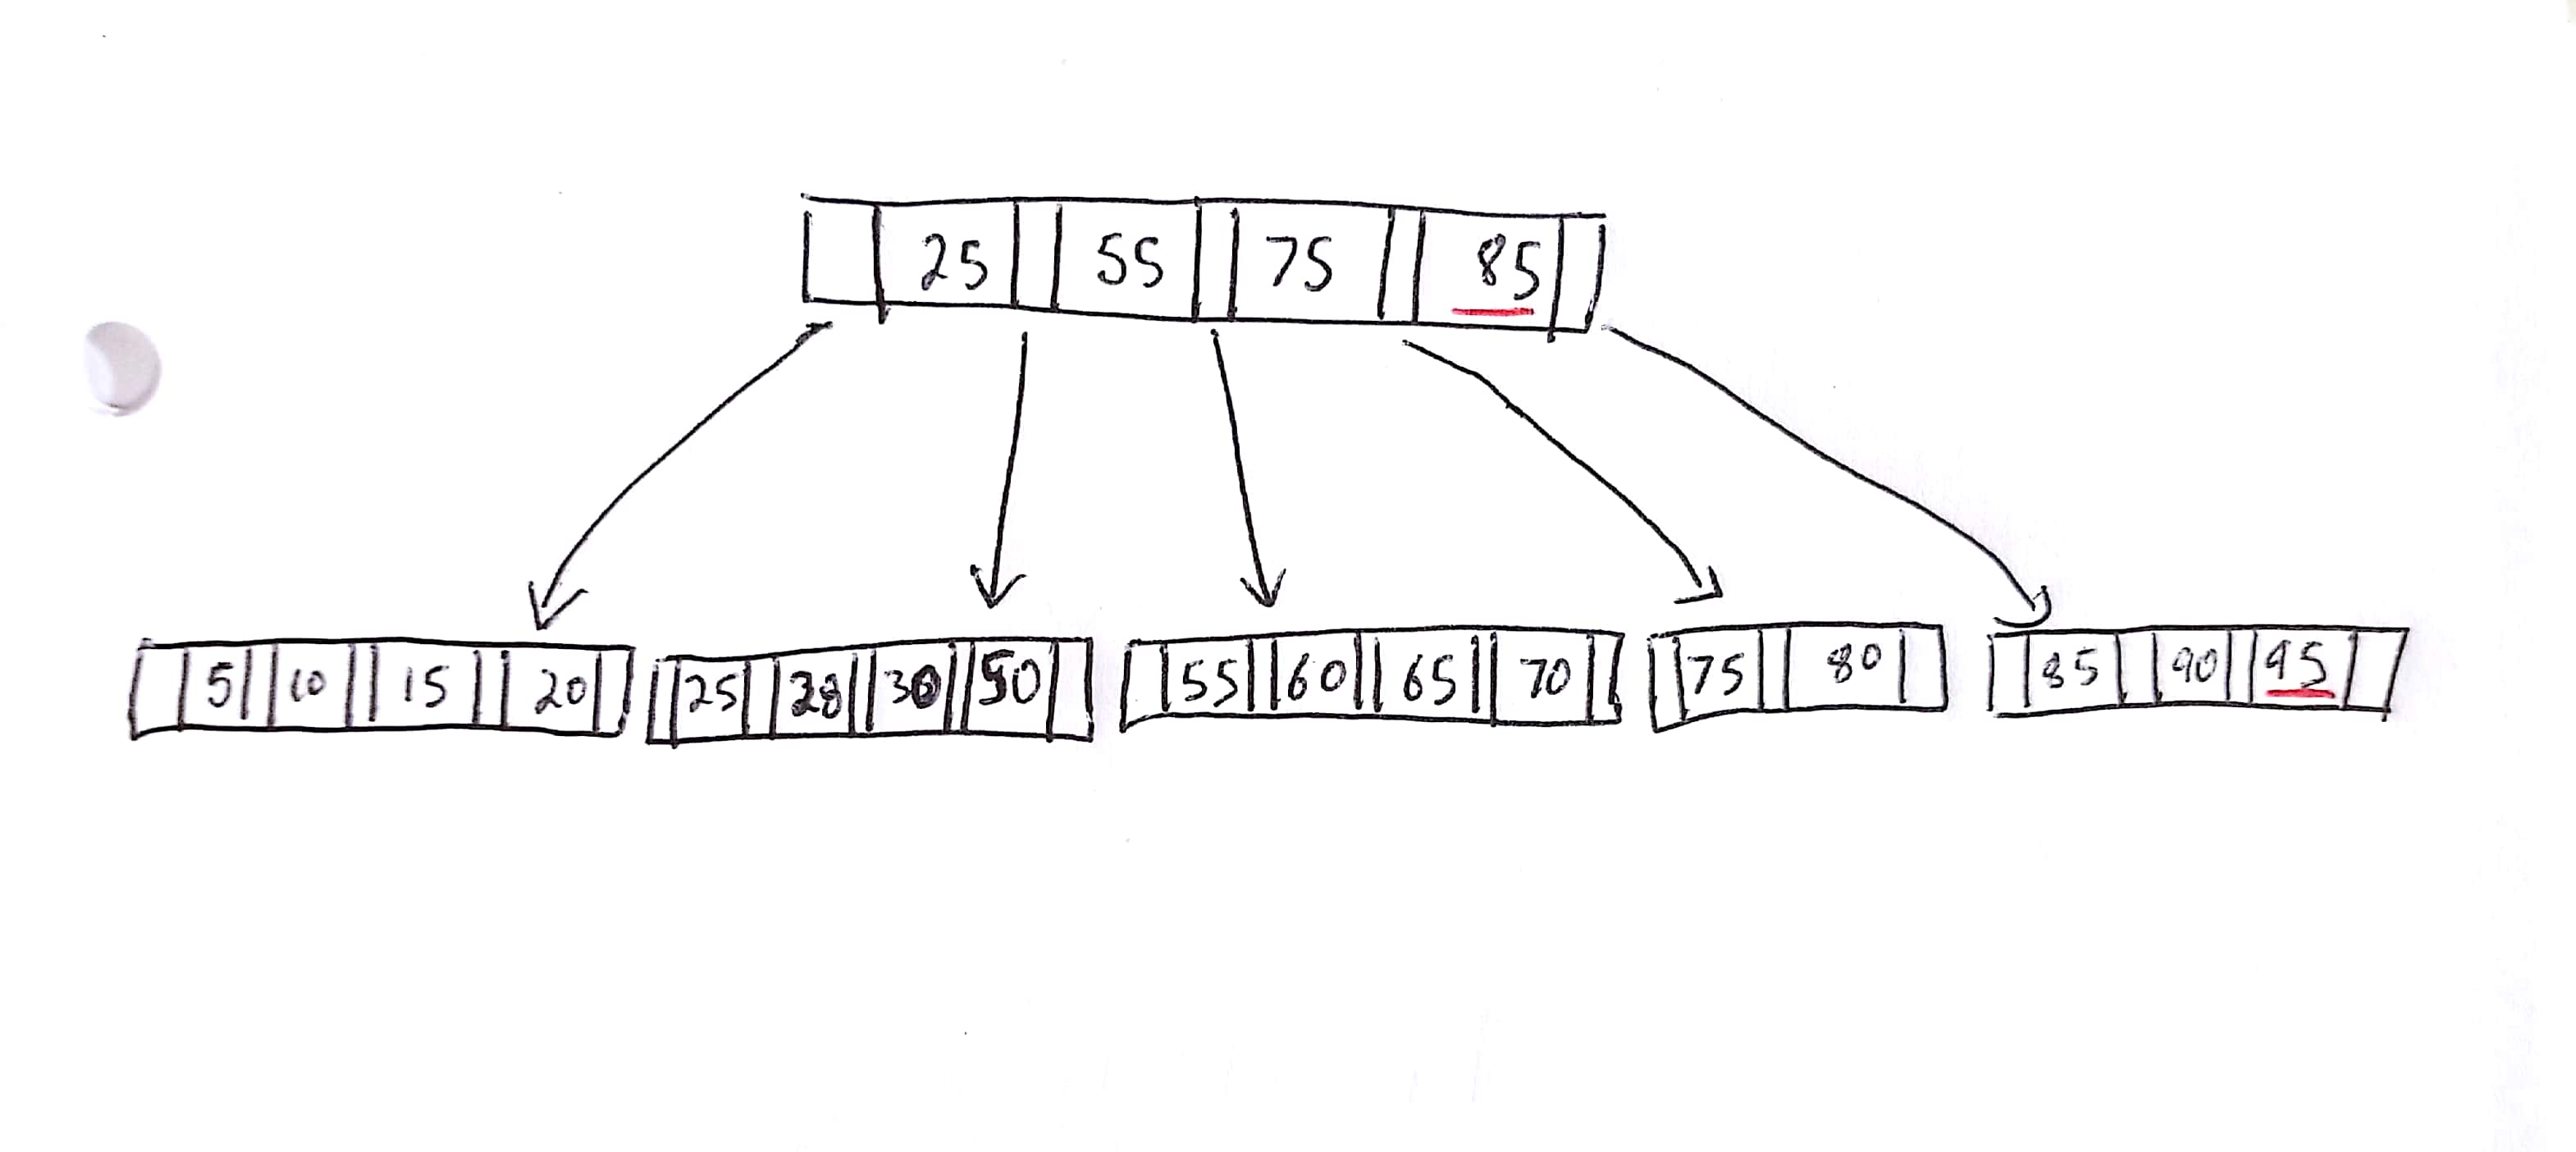
\includegraphics[width=0.9\columnwidth]{figure_q2_1.png}
		\caption{Tree for question 2.1}
		\label{figure:q2.1}
	\end{figure}

	\item Use the result/solution tree from (1) and Show the B+ tree that would result from deleting the record with search key 60.\\

	\begin{figure}[H]
		\centering
		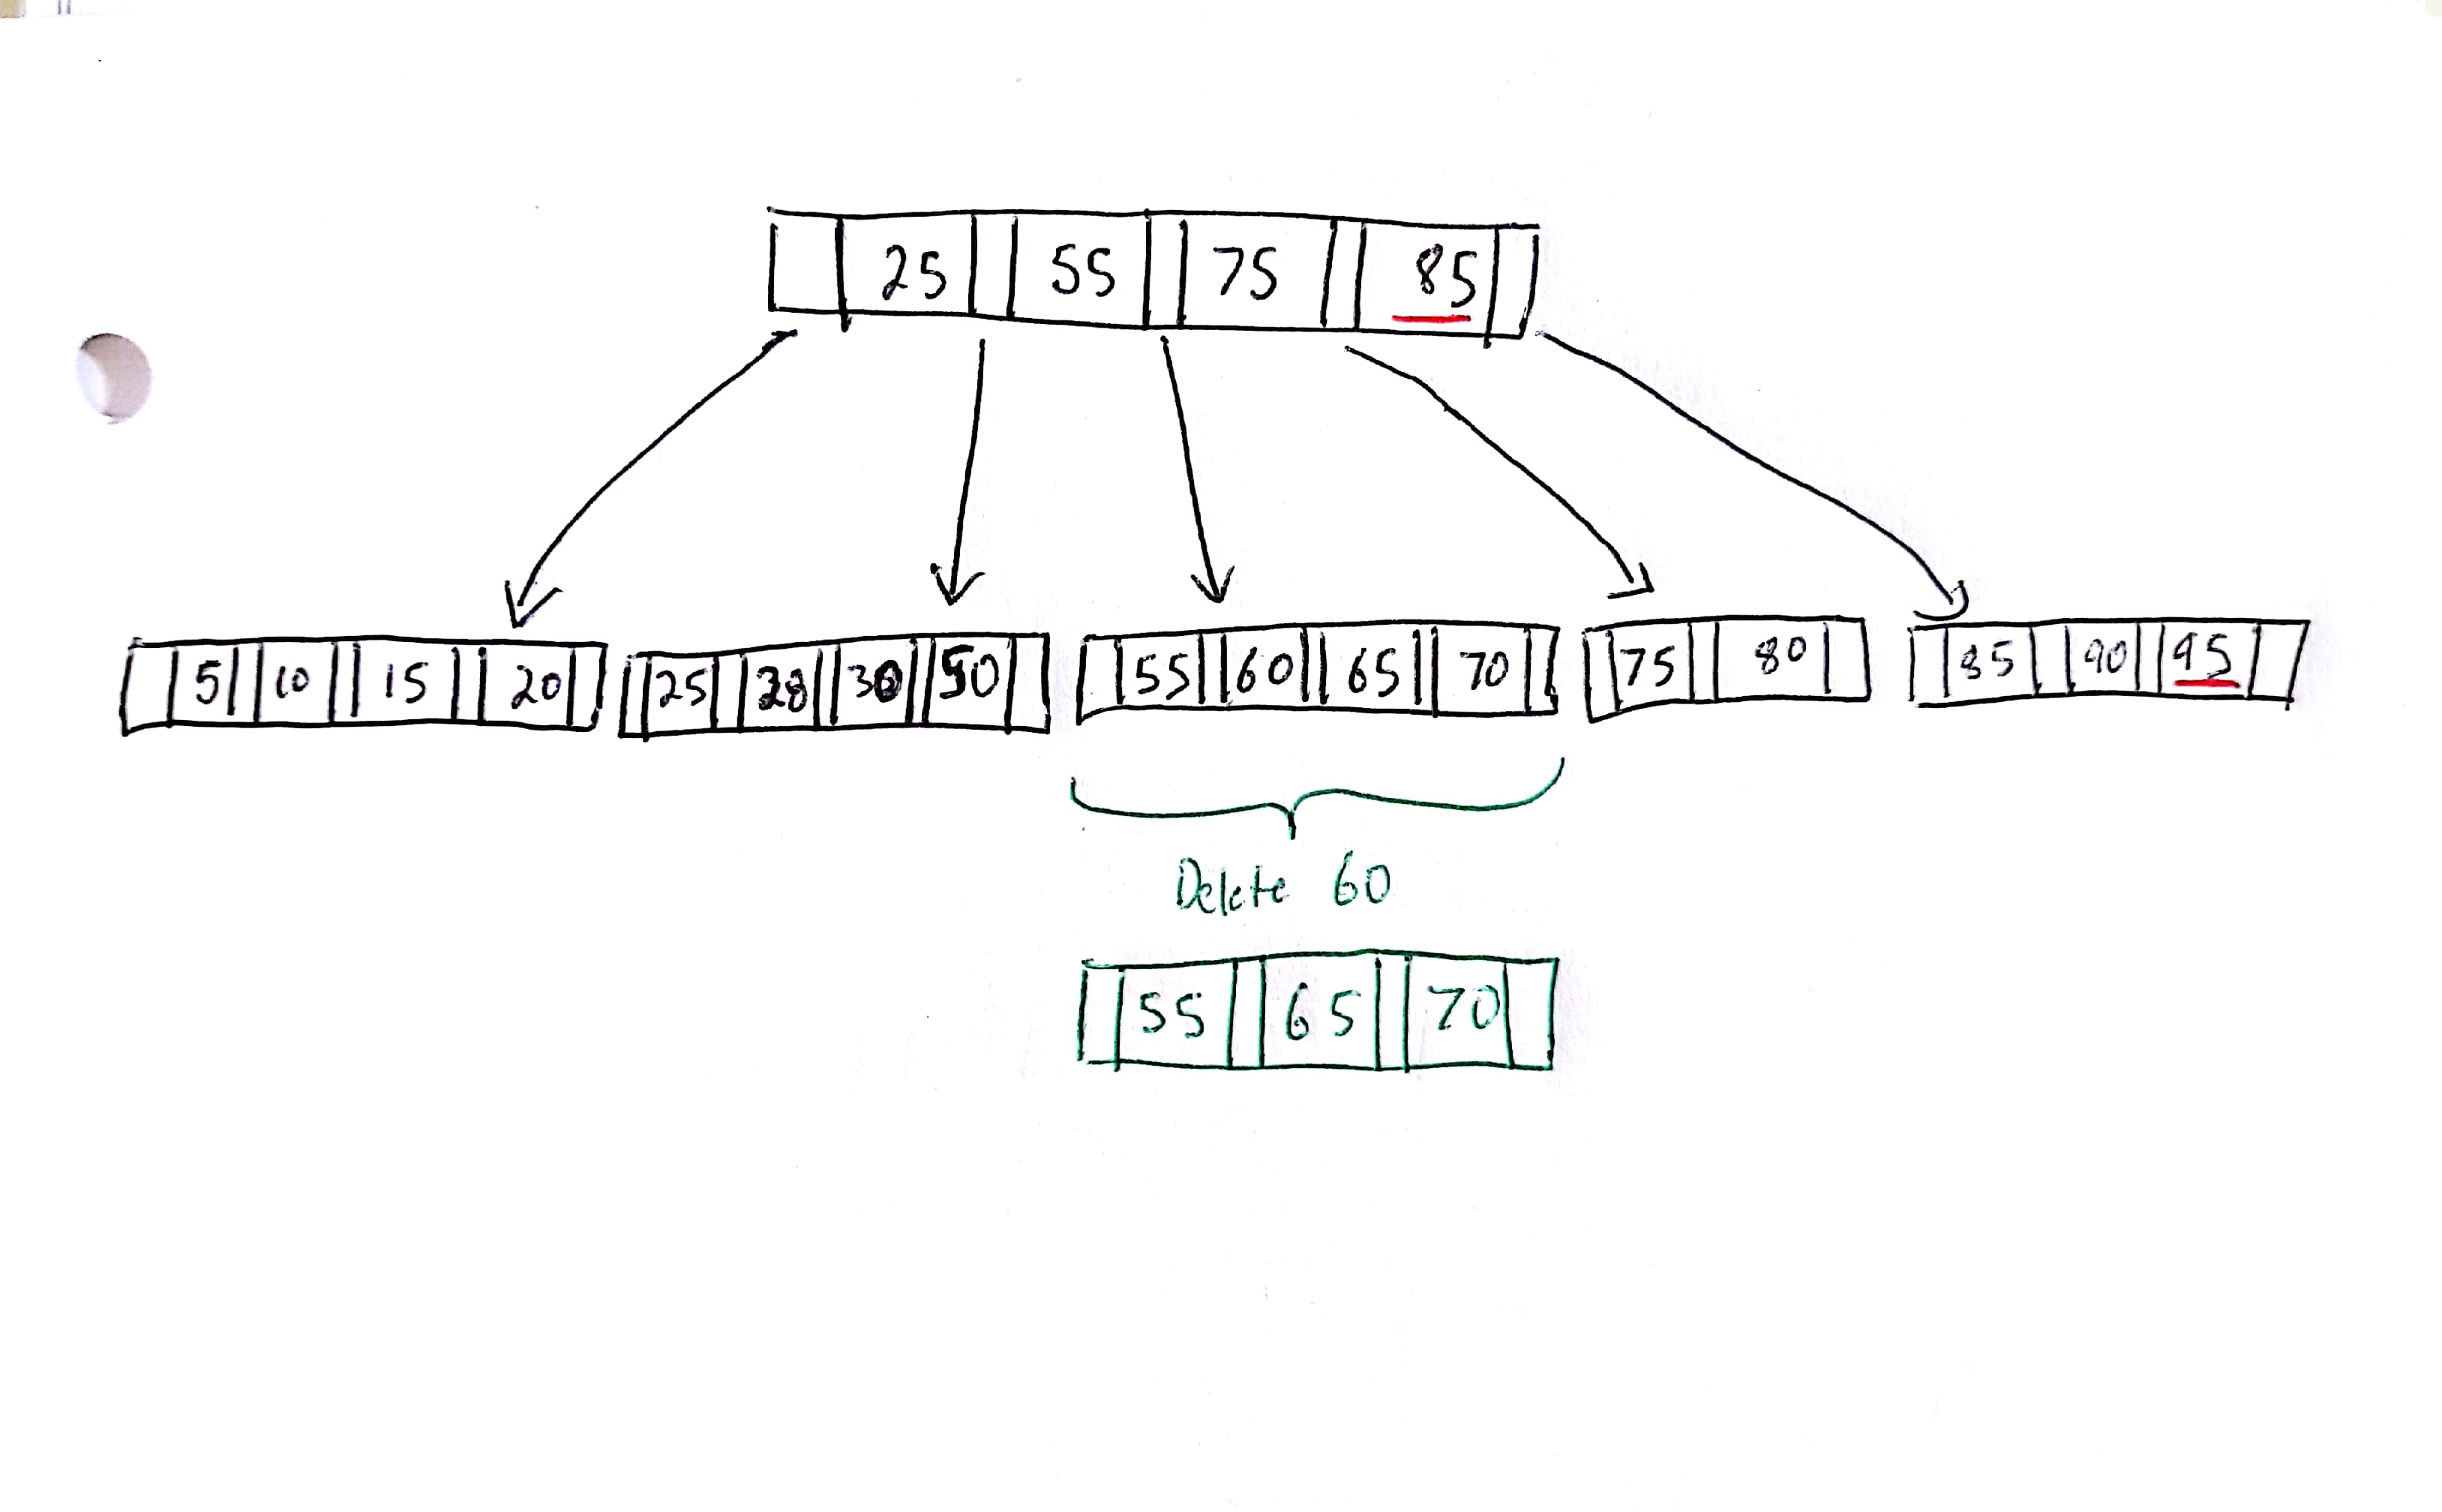
\includegraphics[width=0.9\columnwidth]{figure_q2_2.png}
		\caption{Tree for question 2.2}
		\label{figure:q2.2}
	\end{figure}

	\item Name a search key value such that inserting it into the result/solution tree from (1) would cause an increase in the height of the tree.\\
	\part{solution}\\
	Any value below 75 would cause the resulting tree to increase in height because all of those nodes in the second layer and the root node are at maximum capacity. Adding another key to the root node would force it to split and hence gain a new root node.

	\item What can you infer about the contents and the shape of A, B and C subtrees?\\
	\part{solution}\\
	We can infer that subtree A contains keys less than 10, subtree B contains keys more than or equal to 10 and less than 20, and subtree C contains keys more than or equal to 20 and less than 30. We can also infer that, since there is one node with 2 keys and one with 4, that d=2 which means A, B, and C each have 2-4 keys and 3-5 pointers in them.

\end{enumerate}


\question{3}{B+ Tree Indexing (1 point)}
Suppose that a block can contain at most four data values and that all data values are integers. Using only B+ trees of degree 2, give examples of each of the following:
\begin{enumerate}
	\item A B+ tree whose height changes from 2 to 3 when the value 60 is inserted. Show your structure before and after the insertion.\\

	\begin{figure}[H]
		\centering
		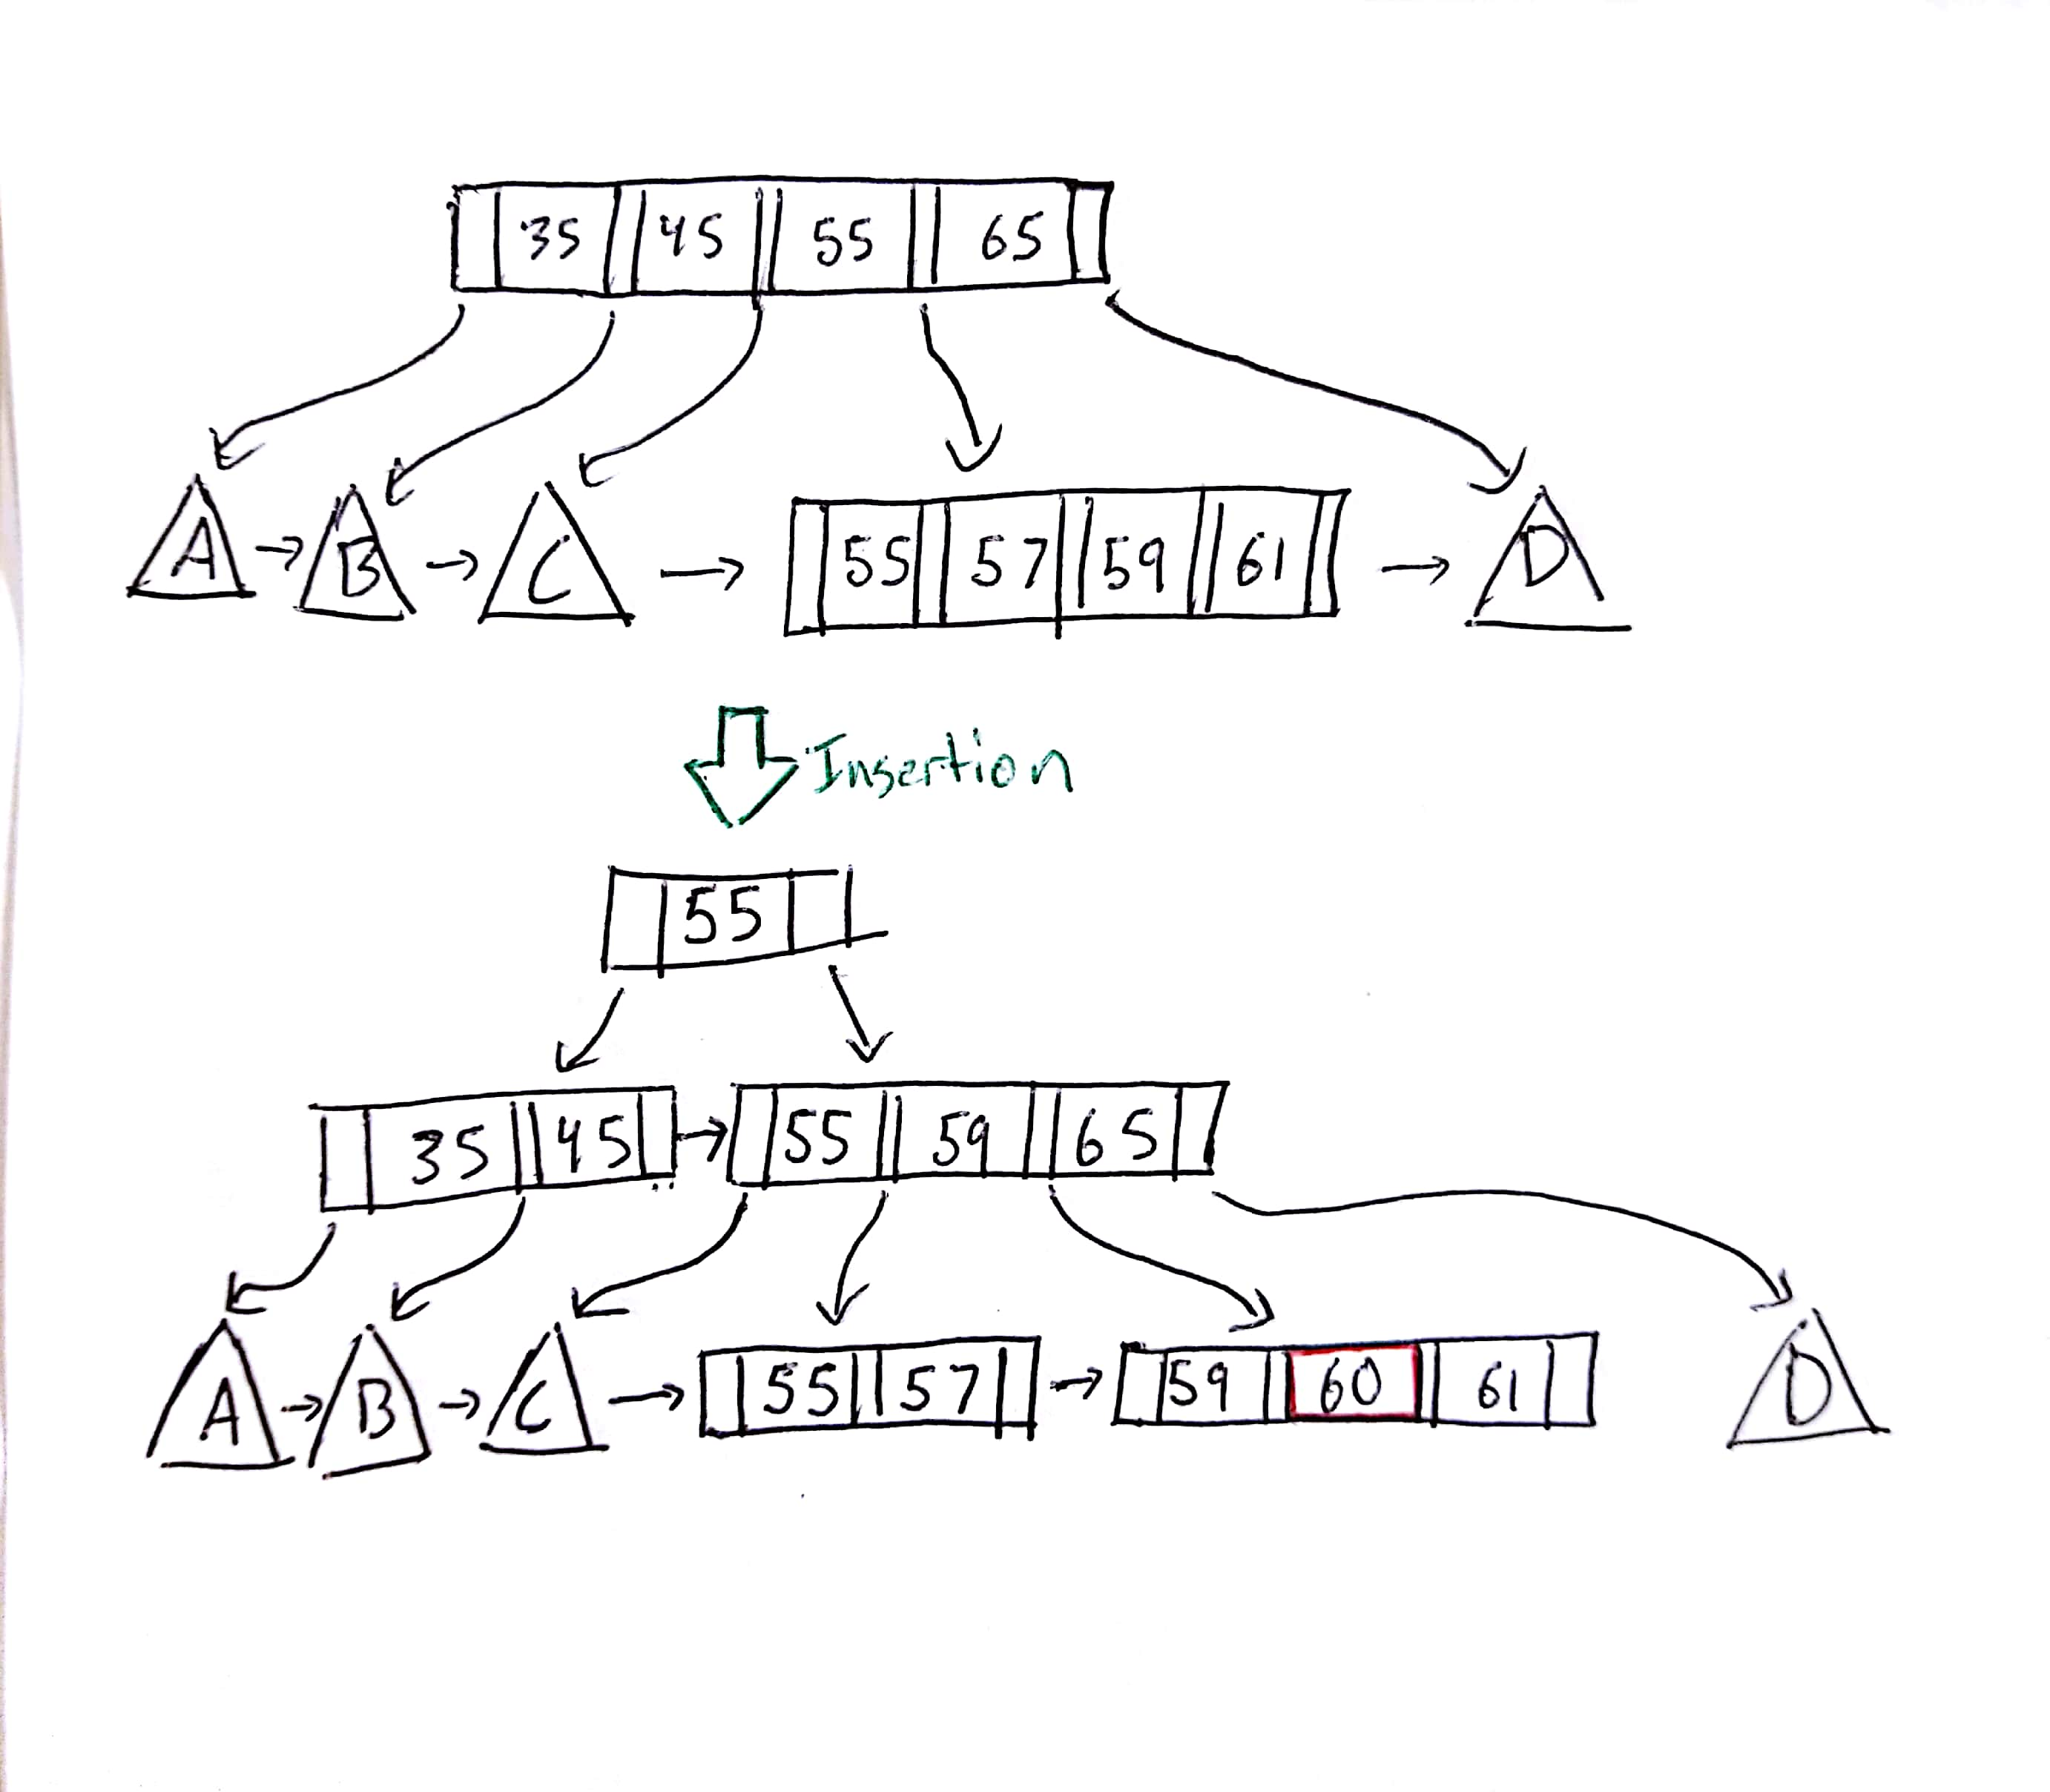
\includegraphics[width=0.9\columnwidth]{figure_q3_1.png}
		\caption{Tree for question 3.1}
		\label{figure:q3.1}
	\end{figure}

	\item A B+ tree in which the deletion of the value 60 leads to a redistribution. Show your structure before and after the deletion.\\

	\begin{figure}[H]
		\centering
		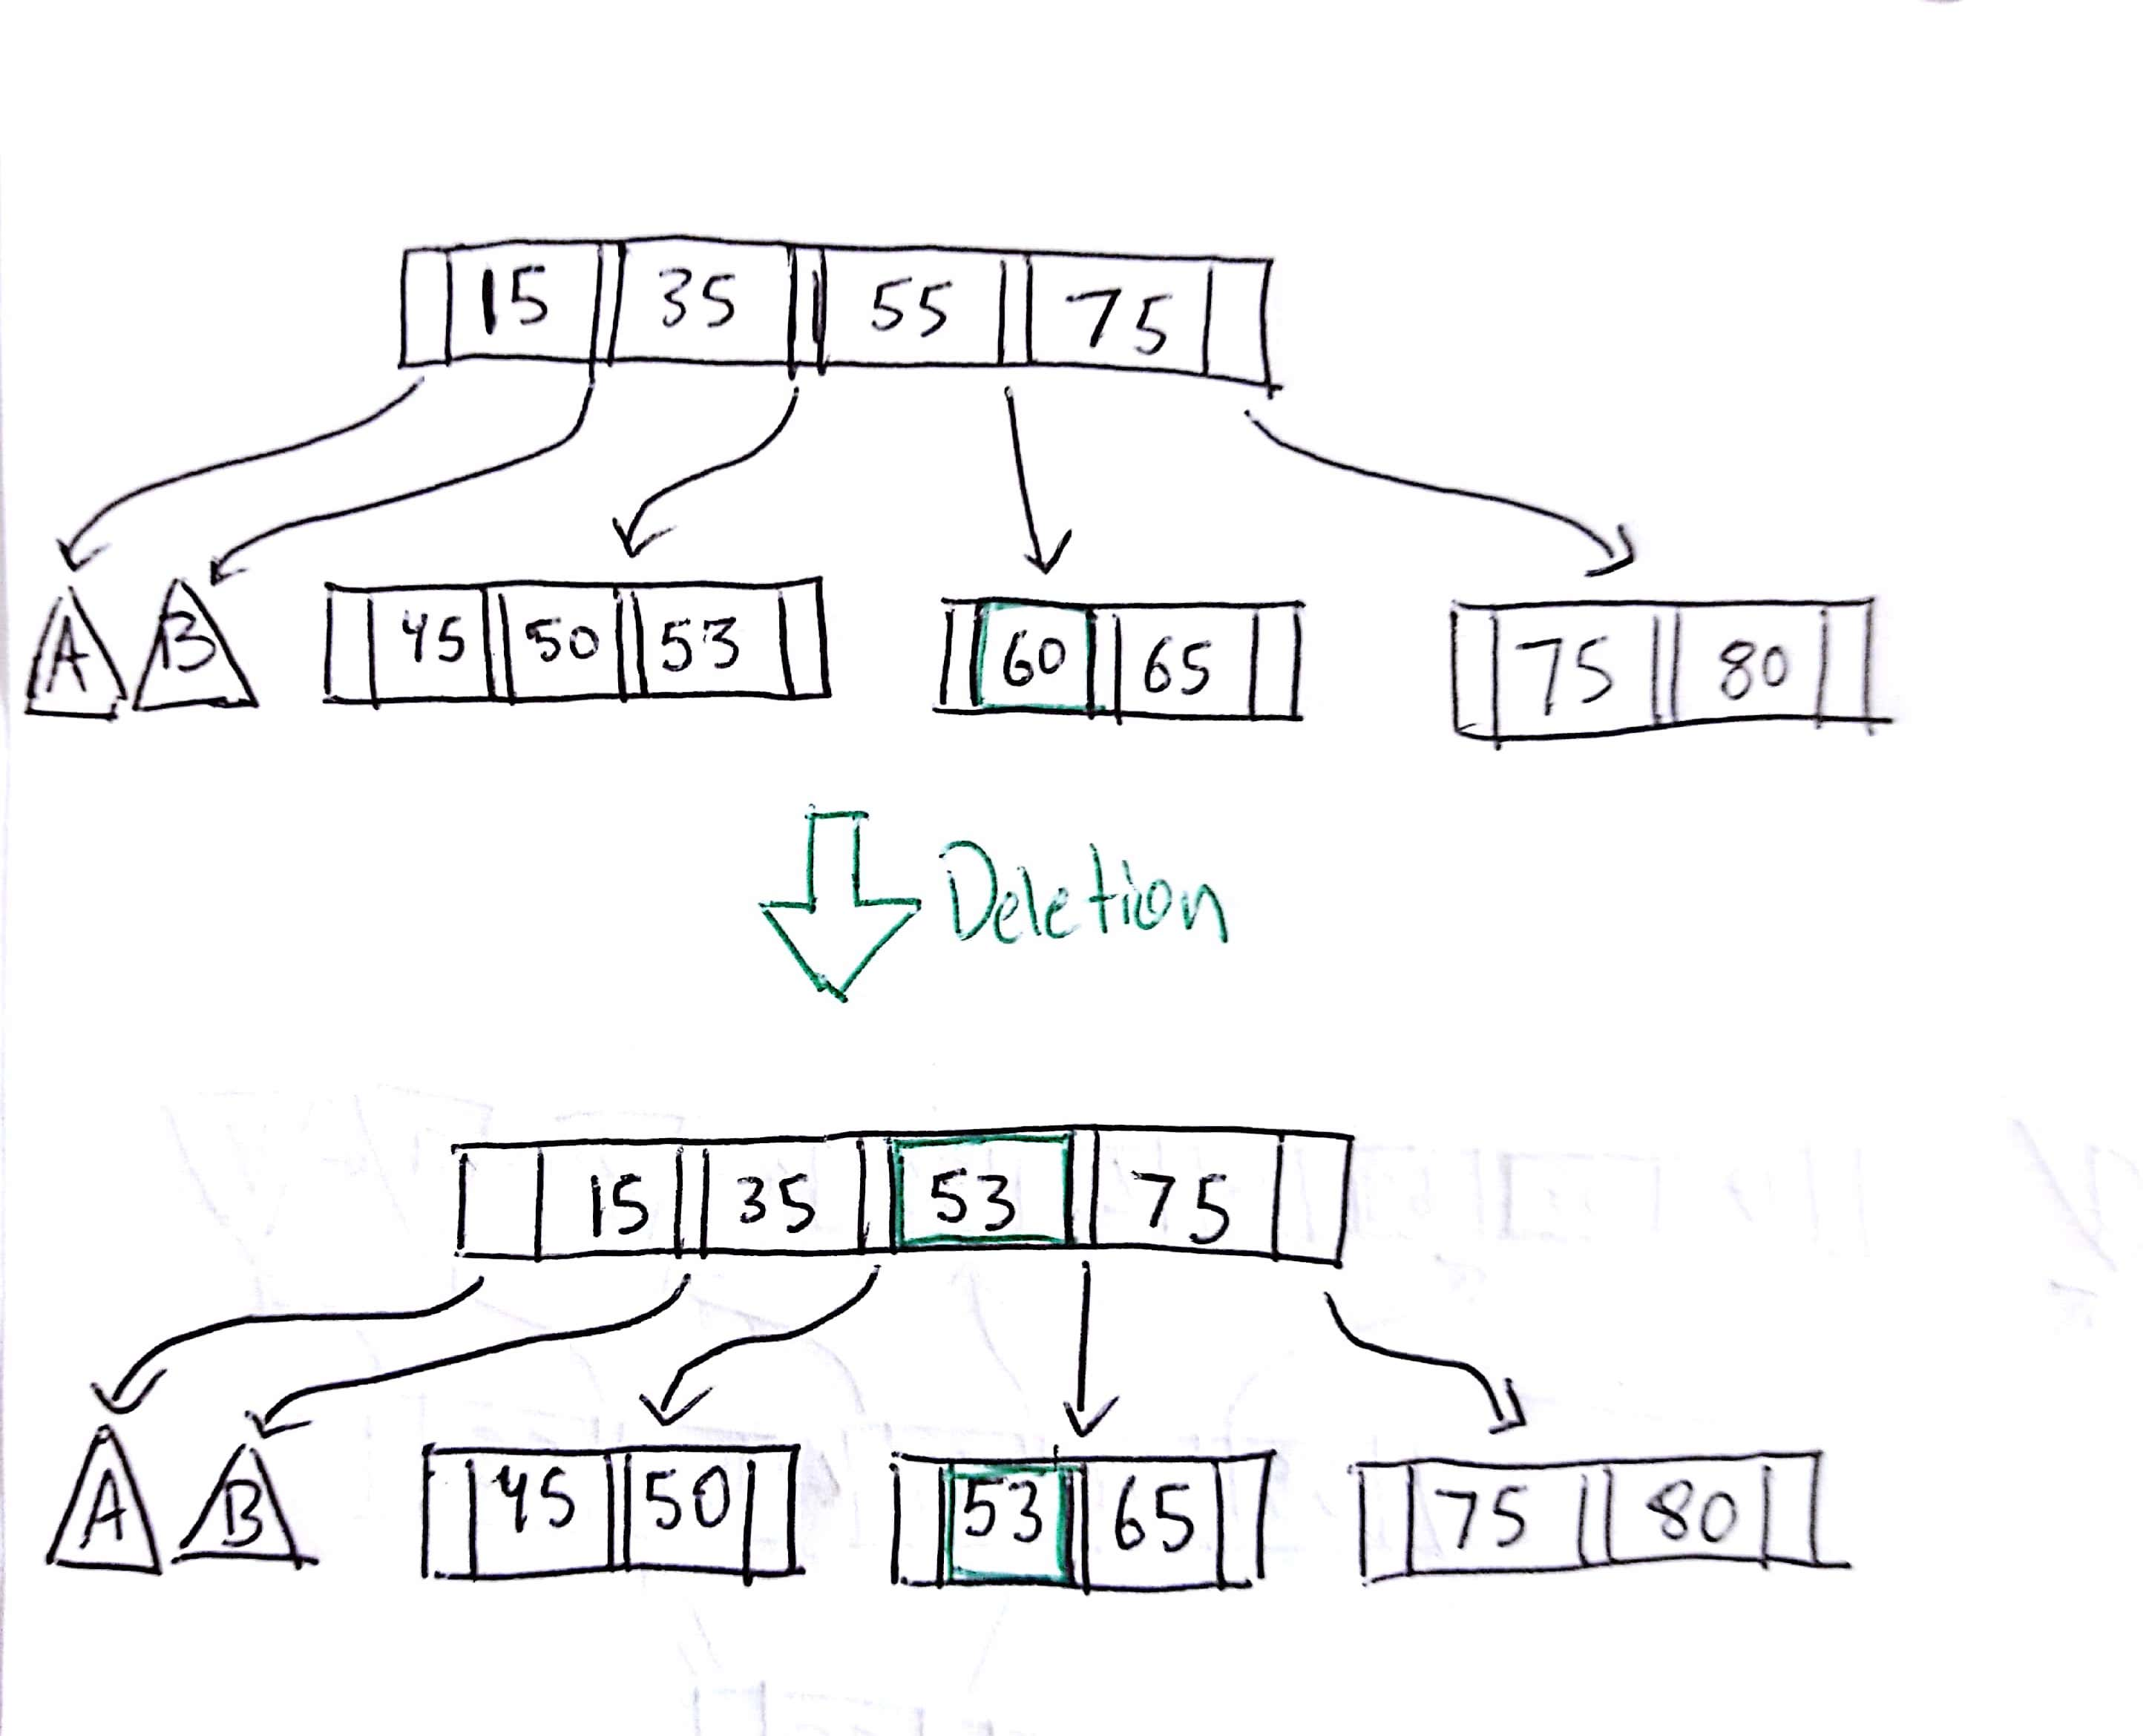
\includegraphics[width=0.9\columnwidth]{figure_q3_2.png}
		\caption{Tree for question 3.2}
		\label{figure:q3.2}
	\end{figure}

%	\item A B+ tree in which the deletion of the value 25 causes a merge of two nodes but without altering the height of the tree.
\end{enumerate}


\question{4}{B+ Tree Indexing (1 point)}
Consider the instance of the Students relation shown.
%Show a B+ tree of degree 2 in each of these cases below.
\begin{enumerate}

	\item To reduce the number of I/O access in index search, each B+ tree node should fit in a block. Let {\it sid} be an integer requiring 16 bits. Let a pointer require 32 bits.
	If the block size is 28 bytes (consisting of 8 bits), what is the maximum degree of the B+ tree index on {\it sid} so each B+ tree node fit in a block?\\
	\part{solution}\\
	(2d)(2 bytes) + (2d+1)(4 bytes) $<$= 28 bytes \\
	4d + 8d + 4 $<$= 28 \\
	12d $<$= 24 \\
	d $<$= 2 \\


	\item Show a B+ tree index on {\it sid} of degree calculated in part 1 for all records.

	\begin{figure}[H]
		\centering
		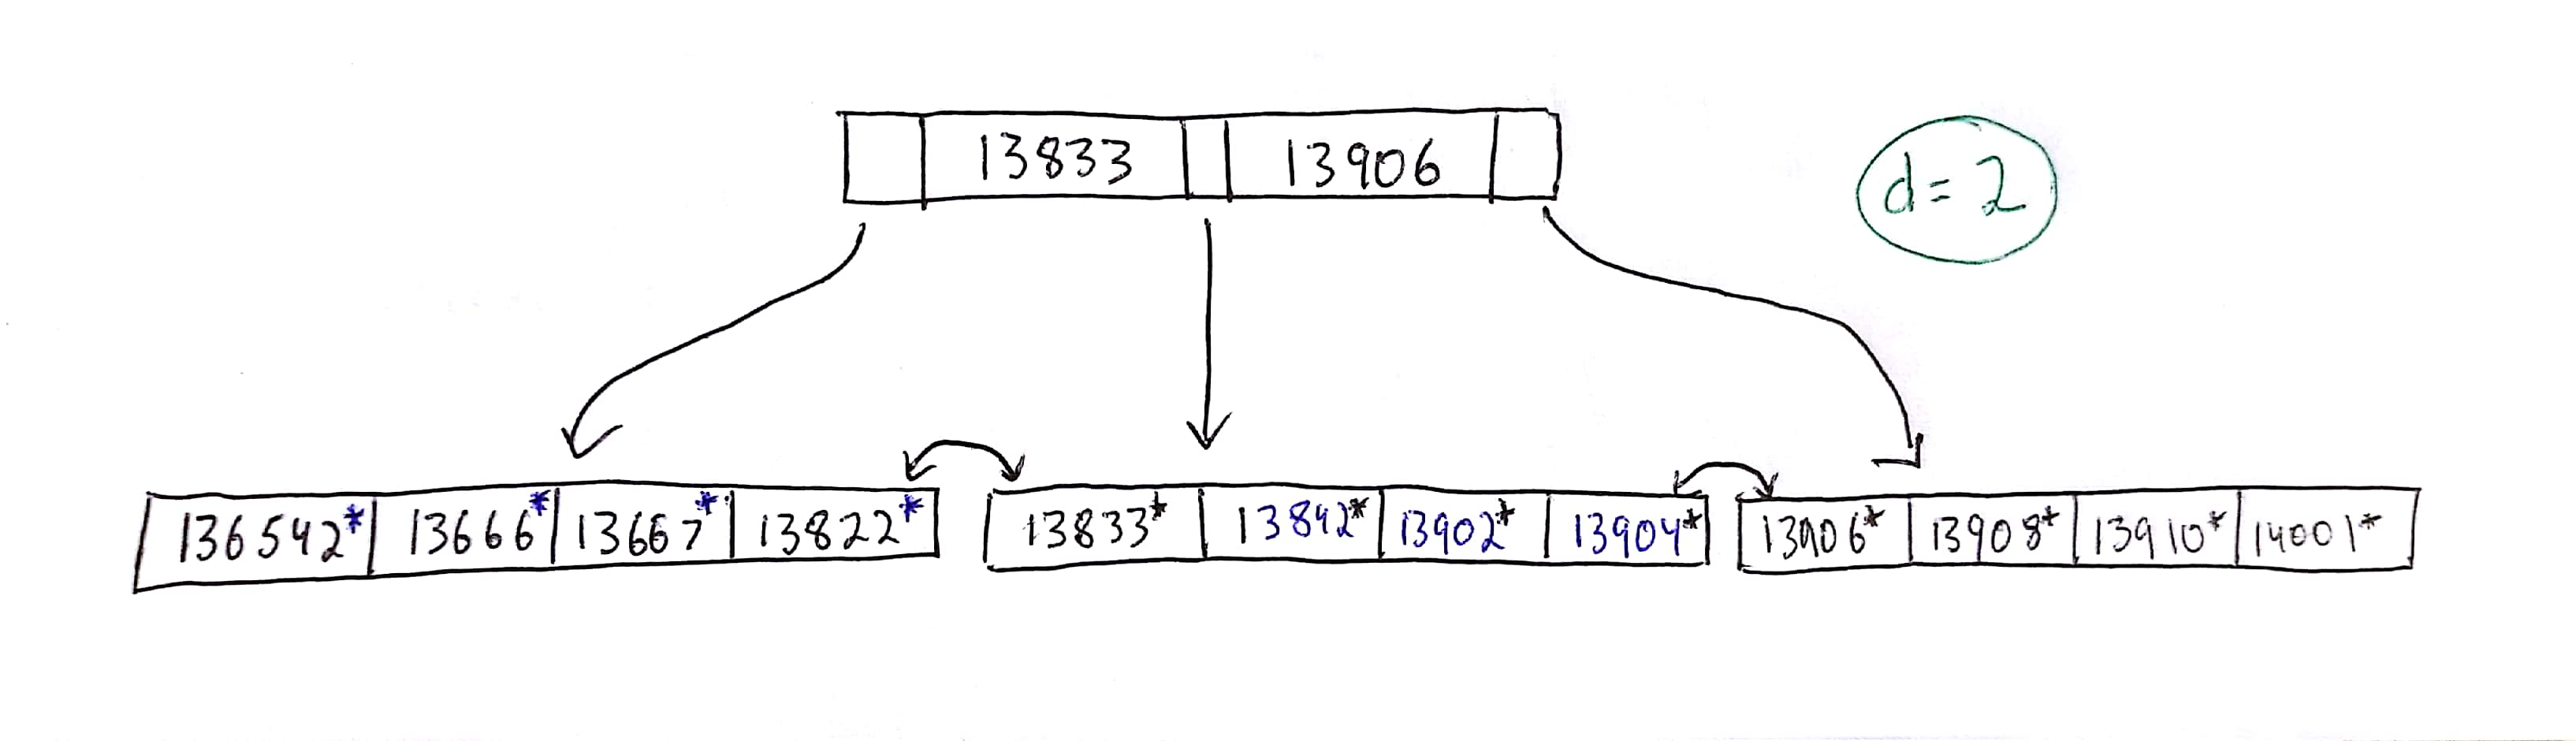
\includegraphics[width=0.9\columnwidth]{figure_q4_2.png}
		\caption{Tree for question 4.2}
		\label{figure:q4_2}
	\end{figure}



%	\item A dense B+ tree index on {\it gpa} where leaf nodes contain
%	the search key and a pair $\left\langle \mathit{pageid}, \mathit{slot} \right\rangle$ to identify a tuple.
%	For this question, assume that these tuples are stored in a sorted file in the order shown in Figure~\ref{figure:question_3}: The first tuple is in page 1, slot 1; the second tuple is in page 1, slot 2; and so on. Each page can store up to {\bf three} data records.
%	For example, the first tuple is represented by ``1.8: $\left\langle 1,1 \right\rangle$''.

\end{enumerate}







\end{document}
